% !TeX spellcheck = en_US
% LaTeX document class
\documentclass[nominted]{uniza}

%-------------------------------------------------------
%             Abbreviation and term database
%-------------------------------------------------------
% !TeX spellcheck = sk_SK

%----------------------------------------------------------
%						Slovník
%----------------------------------------------------------

\DeclareAcronym{viskozita} {
	short = Viskozita,
	long = {Fyzikálna veličina, miera odporu tekutiny deformovať sa pod vplyvom šmykových (tangenciálnych) napätí. Prejavuje sa vnútorným trením.},
	class = dict
}

\DeclareAcronym{zhlukovanie} {
	short = Zhlukovanie,
	long = {Trieda metód strojového učenia, ktoré v daných dátach hľadajú zhluky.},
	extra = {\begin{subdict}
			\item[Hierarchické zhlukovanie] Metódy zhlukovania, kde rozdelenie do zhlukov má hierarchickú štruktúru.
			\item[Fuzzy c-means zhlukovanie] Verzia algoritmu k-means pre fuzzy zhlukovanie.
		\end{subdict}
	},
	class = dict
}

\DeclareAcronym{triedenie} {
	short = Triedenie,
	long = {Pojmy v slovníku sa automaticky triedia podľa abecedy. \hl{Ale pozor: triedenie sa deje prvého argumentu makra \texttt{DeclareAcronym} -- nie podľa poľa \texttt{short}.}},
	class = dict
}

\DeclareAcronym{slovnik_pojmov} {
	short = Slovník pojmov,
	long = {\hl{Slovník pojmov je nepovinný. Na jeho odstránenie stačí zmazať všetky zadefinované pojmy v súbore modules/abbterms.tex.}},
	class = dict
}

%----------------------------------------------------------
%						Skratky
%----------------------------------------------------------

\DeclareAcronym{MAE} {
	short = MAE,
	long = stredná absolútna chyba (\angl{mean absolute error}),
	class = abbrev
}

\DeclareAcronym{ANN} {
	short = ANN,
	long = umelá neurónová sieť (\angl{artificial neural network}),
	class = abbrev
}

\DeclareAcronym{MLP} {
	short = MLP,
	long = {viacvrstvový perceptrón, viacvrstvová neurónová sieť (\angl{multi-layer perceptron})},
	class = abbrev
}


%-------------------------------------------------------
%            Súbory s bibliografickými informáciami
%-------------------------------------------------------
\addbibresource{bibliography.bib}

%-------------------------------------------------------
%                  Jazykové nastavenia
%-------------------------------------------------------
\usepackage[english,slovak]{babel}

%-------------------------------------------------------

%                Informácie o dokumente
%-------------------------------------------------------

\title{Realizing walking for a walking robot using deep reinforcement learning}
\subtitle{*The name is a placeholder until I get official english name}
\author{Bc., Daniel Adamkovič}
\keywords{robotics, deep reinforcement learning, artificial intelligence, simulation}
\keywordsSecLang{robotika, hlboké učenie s odmenou, umelá inteligencia, simulácia}

\keywordsName{Keywords}
\keywordsNameSecLang{Kľúčové slová}

\faculty{Faculty of Electrical Engineering and Information Technology}
\department{Department of Control and Information Systems}

% školiace pracovisko, ak je iné než katedra:
%\supervisorinst{
%	SIEMENS\\
%	Kompetenčné centrum Žilina
%}

\facultyshort{FEIT}
\location{Žilina}

\doctype{Master thesis}
\docid{69 69 420}
\supervisor{Ing. PhD., Michal Gregor}


\academicyear{2020/2021} % akademický rok
\submissionyear{2020} % rok odovzdania práce
% Študijný program:
\studyprogramme{Cybernetics}
% Študijný odbor:
\fieldofstudy{5.2.14 Automation}

% Abstrakt v hlavnom jazyku
\abstract{Abstract}{
Abstrakt obsahuje informáciu o cieľoch práce, jej stručnom obsahu a v závere abstraktu sa charakterizuje splnenie cieľa, výsledky a význam celej práce. Abstrakt sa píše súvisle ako jeden odsek a jeho rozsah je spravidla 100 až 500 slov.
}

% Abstrakt v cudzom jazyku (anglickom, nemeckom, ...)
\abstractSecLang{Abstrakt}{
Nejaký abstrakt po slovensky.
}

\date{Dátum odovzdania práce}

\acknowledgements{
	Poďakovanie nie je povinné. Ak nemá byť zahrnuté, stačí túto časť zakomentovať.
}

%-------------------------------------------------------
%		 Vybrané metadáta zapíšeme aj do dokumentu.
%-------------------------------------------------------

\hypersetup{
	pdfauthor={\Author},%
    pdftitle={\Title},%
    pdfsubject={\Doctype},%
    pdfkeywords={\Keywords},%
    pdfproducer={LaTeX},%
%    pdfcreator={pdfLaTeX}
}

%-------------------------------------------------------
%						Includeonly
%-------------------------------------------------------

%\includeonly{
%kap_uvod
%}

%-------------------------------------------------------
%		Korektné zalamovanie spojok na konci riadku.
%-------------------------------------------------------
%\usepackage{encxvlna}
% a temporary workaround for encxvlna breaking multiarg macros


%-------------------------------------------------------
%					Začiatok dokumentu
%-------------------------------------------------------

\begin{document}

%-------------------------------------------------------
%				 Obálka a titulná strana
%-------------------------------------------------------

\makecover
\maketitle

%-------------------------------------------------------
%						 Zadanie
%-------------------------------------------------------

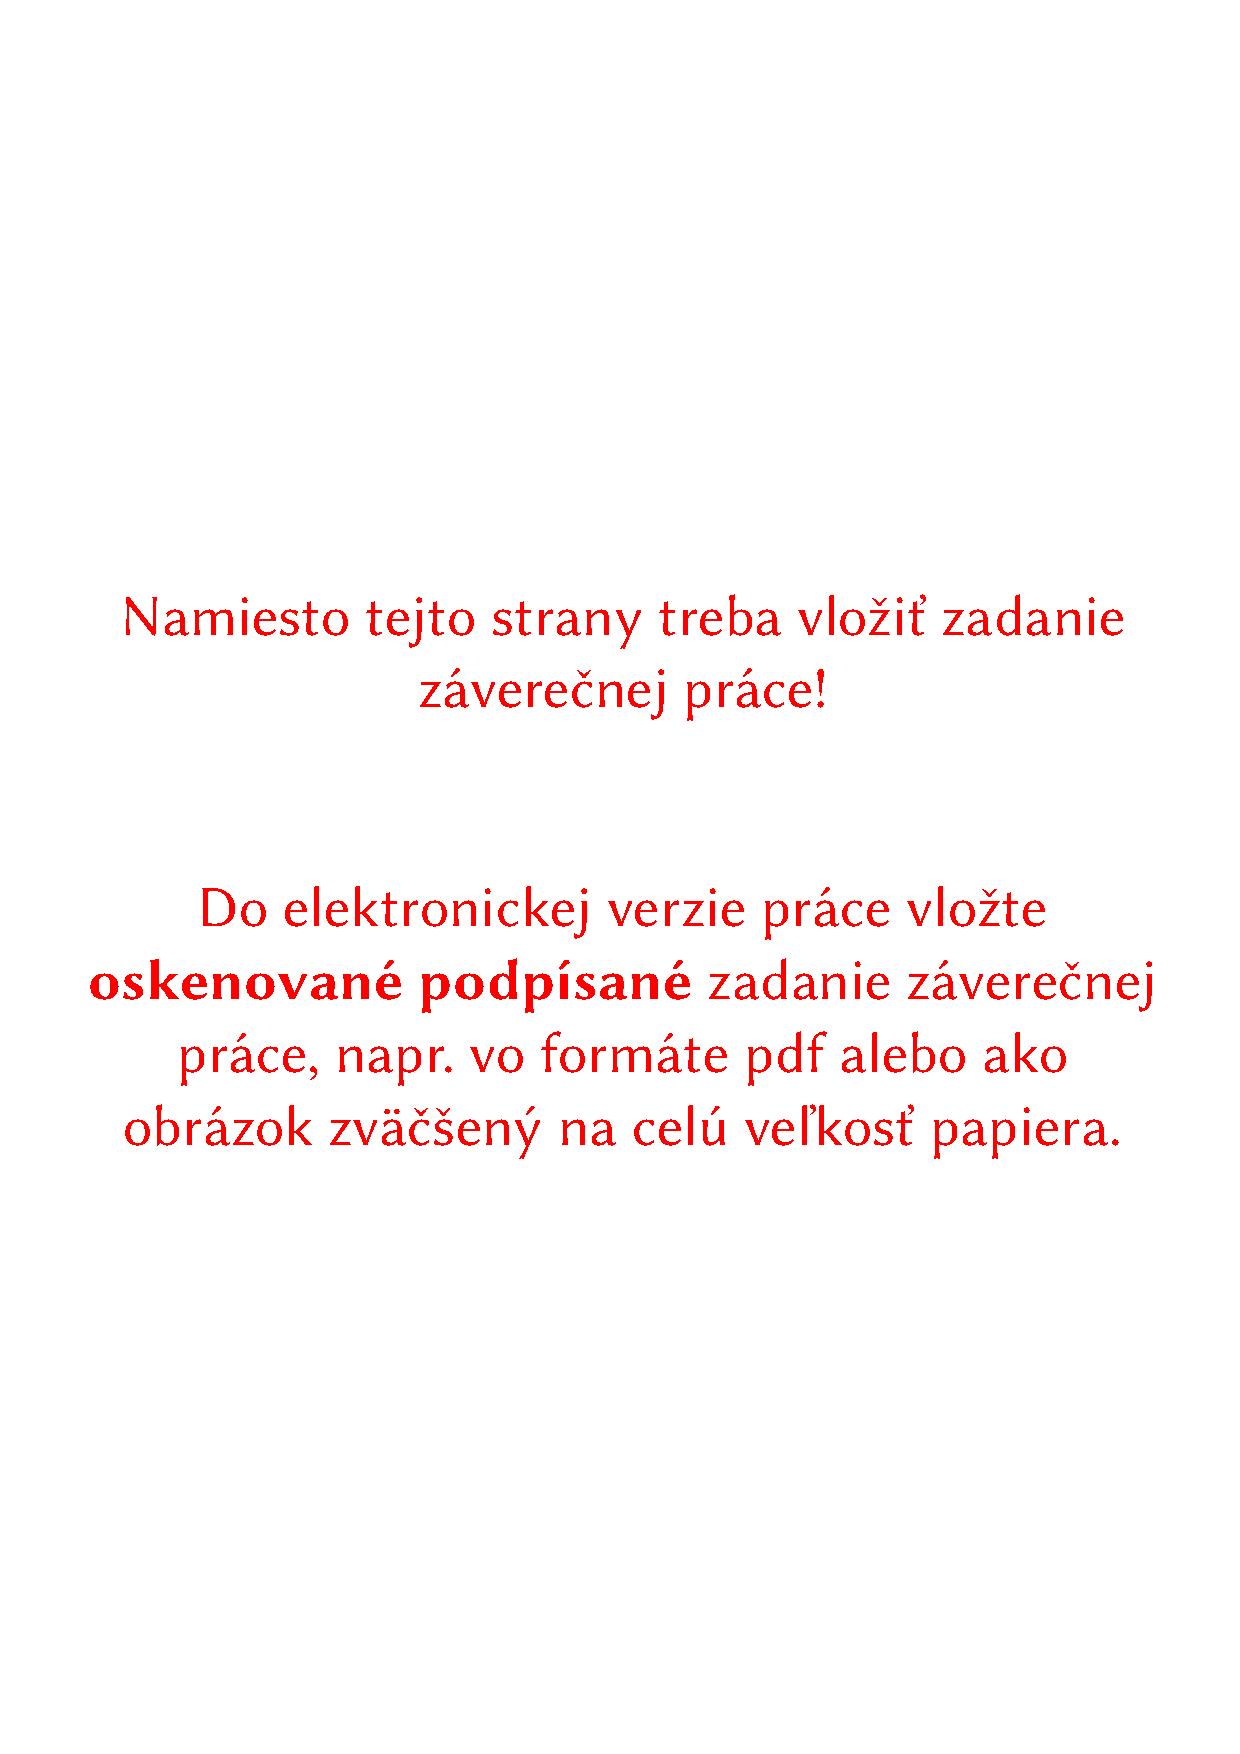
\includepdf[fitpaper]{modules/zadanie.pdf}

%-------------------------------------------------------
%				Front Matter (TOC, LOF, ...)
%-------------------------------------------------------
\frontmatter

% suppress some commands in TOC and lists
\begingroup
\renewcommand{\ac}[1]{#1}
\renewcommand{\cite}[1]{}

% Poďakovanie
\makeacknowledgements

% Abstrakt, anotácia
\makeabstract

%  TOC
\tableofcontents

% list of figures
\iftotalfigures\listoffigures\fi

% list of tables
\iftotaltables\listoftables\fi

% list of abbreviations
\acsetup{page-ref=comma,list-style=acronyms
}{
	\ifargoutempty{\printacronyms[include-classes=abbrev,heading=none]}{}{
		\unchapter{Abbreviations}
		\argoutemptyFirstArg
	}
}

% dictionary
\acsetup{page-ref=none,list-style=dictstyle,extra-style=plain,extra-format={\;},only-used=false}{
\ifargoutempty{\printacronyms[include-classes=dict,heading=none]}{}{
	\unchapter{Dictionary of terms}
	\setlength{\columnseprule}{0.2pt}
	\setlength{\columnsep}{1.25cm}
	\begin{multicols}{2}
	\argoutemptyFirstArg
	\end{multicols}
}}

\endgroup % suppress some commands in TOC and lists

%-------------------------------------------------------
%						Document
%-------------------------------------------------------
\mainmatter

% !TeX spellcheck = en_US
\chapter{Introduction}


In the last couple of decades we have witnessed many groundbreaking developments that would have previously been reserved for science fiction. Modern mobile robots can walk, interact with objects and humans, even independently accomplish simple tasks previously only reserved for humans. However while the robots are becoming more complex by the year, so does the complexity of their design and development. This is most obvious with robots that utilize legs for the purposes of locomotion, which forces engineers to develop complex controllers that allow such machines to move about. Design of these controllers is more often than not non-trivial and as such it is often reserved for experienced control engineers. Still, even with a lot of effort success is not guaranteed and even well-designed robots rarely achieve the same grace of movement that animals are capable of.

With this paragraph we have formulated the problem that this thesis addresses. For one way of solving it we can, as engineers often do, draw inspiration from nature. An animal learns to walk, not by performing a deep analysis of its tendons and muscles and then committing months to study of books on control theory. No, an animal learns in a much more straightforward way by simply making attempts and attempting to achieve 'good results'. We write good results in quotation marks as measuring goodness of something can be in practice a difficult and often very subjective task. Regardless, this simple concept of making attempts and obtaining a measure of success is, not only present in nature, it is also at the core of one of the most promising sub-fields of artificial intelligence known as reinforcement learning (\ac{RL}). 

\newpage

In this text we will focus on:
\begin{enumerate}[leftmargin=2cm]
\item \textbf{Introducing deep reinforcement learning (\ac{DRL}) algorithms}: with \ac{RL} maturing as a field a slew of different approaches at utilizing it become available. We will explore some of the most promising ones that are relevant for our use case. 
\item \textbf{Simulation and modeling of a robot, task and reward}: just having an algorithm that works is not enough, so this chapter will be dedicated to creating a simulated environment within which we will train a virtual robot to walk.
\item \textbf{Implementing the \ac{DRL}}: \todo[inline]{When I know more about the implementation details I need to modify this} 
\item \textbf{Training and results analysis}: this chapter will be dedicated to putting everything together and analyzing the obtained results.
\item \textbf{Transitioning into the real world}: \todo[inline]{See the comment above}
\end{enumerate}


% !TeX spellcheck = en_US
\chapter{Deep reinforcement learning}
In this chapter we will put \ac{DRL} into the context of broader field of artificial intelligence and explain how it differs from other approaches that attempt to infuse agents with some form of intelligence. Afterwards we will proceed to introduce the main algorithms that are relevant for the use in environments with continuous action spaces.  
\section{DRL in the context of AI}



%-------------------------------------------------------
%                     Bibliography
%-------------------------------------------------------

\printbibliography[heading=unchapter,title={Zoznam použitej literatúry}]

%-------------------------------------------------------
%					Čestné vyhlásenie
%-------------------------------------------------------

\makeDeclaration

%-------------------------------------------------------
%						Appendix
%-------------------------------------------------------

\makeAppendixPage
\appendix

% !TeX spellcheck = sk_SK

\chapter{Zeleninový šalát}

Tvorba príloh je veľmi jednoduchá -- stačí ich pridať ako nové kapitoly v časti dokumentu označenej ako \texttt{{\textbackslash}appendix}. Prílohy sú automaticky číslované nie numericky, ale písmenami abecedy, čím sú dostatočne odlíšené od klasických kapitol. Ak práca obsahuje prílohy, šablóna automaticky vygeneruje titulný list oddeľujúci prílohovú časť práce od hlavnej časti práce.

\section{Textová vata}

\Blindtext


\end{document}
